{\textbf{1. 深度优先搜索遍历(DFS)}}

{从图中的某结点v开始访问,访问他的任意一个邻结点w1;再从w1出发,访问与w1邻接但是没有被访问过的结点w2;然后再从w2出发,进行类似的访问\ldots{}\ldots{},如此进行下去,当一个顶点的所有邻接结点都被访问过时,则依次退回到前一次刚访问过的结点,看是否还有其他没有被访问的邻接结点。如果有,则访问此结点,然后再从此结点出发,进行与前述类似的访问。重复上述过程,直到连通图中所以结点都被访问过为止。}

{图的深度优先搜索遍历类似于二叉树的先序遍历,唯一的区别在于:{二叉树的先序遍历对于每个结点要递归地访问两个分支,图的深度优先搜索遍历则是要递归地访问多个分支。}}

{以邻接表为存储结构的深度优先搜索遍历算法:}

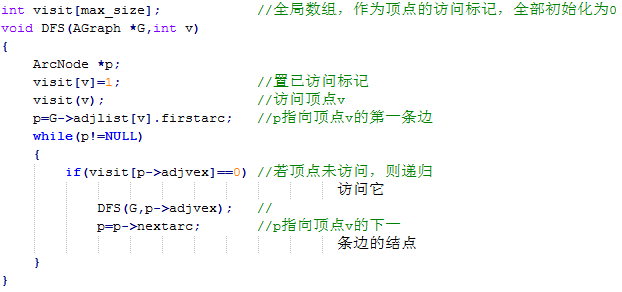
\includegraphics[width=3.70833in,height=1.73958in]{png-jpeg-pics/707E925EDD4194753E9B149C6EFC6D8E.png}

{\textbf{2. 广度优先搜索遍历(BFS)}}

{从图中某个顶点v出发,并访问该顶点,然后访问v的各个未曾被访问的邻接点w1,w2,\ldots{}
,wk,然后依次从w1,w2,\ldots{}
,wk出发访问各自未被访问的邻接点。重复步骤2,直到全部顶点都被访问为止。}

{以邻接表为存储结构的广度优先搜索遍历算法:}

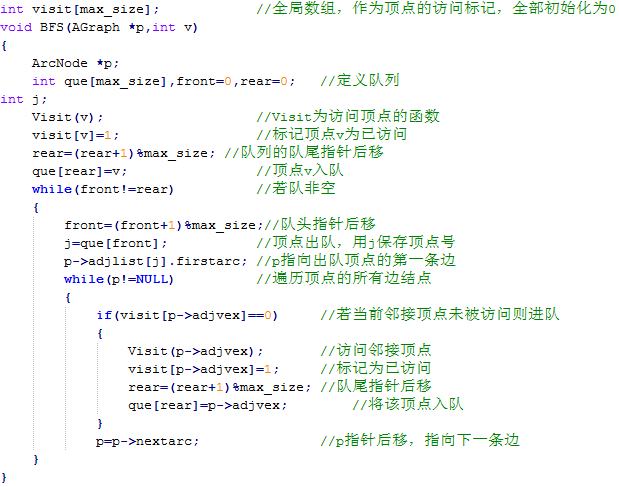
\includegraphics[width=3.70833in,height=2.91667in]{png-jpeg-pics/7BFE384E1625FF63709604A860D8BAAF.png}
